\documentclass[letterpaper]{article}
\usepackage[utf8]{inputenc}
\usepackage[parfill]{parskip}    % Activate to begin paragraphs with an empty line rather than an indent
\usepackage{graphicx}
\usepackage{amssymb}
\usepackage{amsmath}
\usepackage{amsthm}
\usepackage{mathtools}

\usepackage{afterpage}

\usepackage{algorithm}
\usepackage{algpseudocode}

\usepackage{verse}

\newtheorem{theorem}{Theorem}[section]
\newtheorem{corollary}{Corollary}[theorem]
\newtheorem{lemma}[theorem]{Lemma}

\theoremstyle{remark}
\newtheorem*{remark}{Remark}

\usepackage{epstopdf}
\usepackage{circuitikz}
\usepackage[separate-uncertainty = true,multi-part-units=single]{siunitx}
\usepackage{booktabs}
\usepackage{enumitem}
\usepackage[toc,page]{appendix}
\usepackage{color}
\usepackage{pgfplots}
\usepackage{pgfplotstable}
\usepackage{caption}
\usepackage{subcaption}
\usepackage{url}
\usepackage{multirow}
\usepackage{makecell}
\usepackage[round]{natbib}   % omit 'round' option if you prefer square brackets
\usepackage{titling}
\usepackage{siunitx}

\usepackage{setspace}
% \doublespacing
\usepackage{float}


\pgfplotsset{compat=1.14}

%  Special math symbols
%       floor, ceiling, angled brackets
%-----------------------------------------------------------------------
\newcommand{\floor}[1]{\left\lfloor #1\right\rfloor}
\newcommand{\ceil}[1]{\left\lceil #1\right\rceil}
\newcommand{\etal}{\textit{et al.}}
\newcommand{\RE}{\mathbb{R}}        % real space
\newcommand{\ZZ}{\mathbb{Z}}        % integers
\newcommand{\NN}{\mathbb{N}}        % natural numbers
\newcommand{\eps}{{\varepsilon}}    % prettier epsilon
%-----------------------------------------------------------------------
%  Tighter lists
%-----------------------------------------------------------------------
\newenvironment{itemize*}% Tighter itemized list
  {\begin{itemize}%
    \setlength{\itemsep}{-0.5ex}%
    \setlength{\parsep}{0pt}}%
  {\end{itemize}}
\newenvironment{description*}% Tighter description list
  {\begin{description}%
    \setlength{\itemsep}{-0.5ex}%
    \setlength{\parsep}{0pt}}%
  {\end{description}}
\newenvironment{enumerate*}% Tighter enumerated list
  {\begin{enumerate}%
    \setlength{\itemsep}{-0.5ex}%
    \setlength{\parsep}{0pt}}%
  {\end{enumerate}}
%-----------------------------------------------------------------------
% Typing shortcuts
%-----------------------------------------------------------------------
\newcommand{\X}{\mathbb{X}}
\newcommand{\SG}{\mathbf{S}}
\newcommand{\GE}{\mathcal{G}}
\newcommand{\ST}{\,:\,}
\renewcommand{\tilde}[1]{\widetilde{#1}}
\newcommand{\diam}{\mathrm{diam}}
\newcommand{\sq}{\square}
\newcommand{\half}[1]{\frac{#1}{2}}
\newcommand{\inv}[1]{\frac{1}{#1}}
\newcommand{\alg}{\textsf{SplitReduce}}
\newcommand{\sz}[1]{\sigma_{#1}}
\newcommand{\LL}{\mathcal{L}}
\newcommand{\softOmega}{\widetilde{\Omega}} 
\newcommand{\softO}{\widetilde{O}}
\newcommand{\OO}{O^*}  %or \widetilde{O}?

\newcommand{\norm}[1]{\left\lVert#1\right\rVert}

\newcommand{\dx}{\mathrm{d}x}
\newcommand{\dy}{\mathrm{d}y}
\newcommand{\dz}{\mathrm{d}z}
\newcommand{\dt}{\mathrm{d}t}
\newcommand{\du}{\mathrm{d}u}
\newcommand{\dtheta}{\mathrm{d}\theta}
\newcommand{\dq}{\mathrm{d}q}
\newcommand{\diff}{\mathrm{d}}
\newcommand{\dV}{\mathrm{d}V}
\newcommand{\dL}{\mathrm{d}L}
\newcommand{\dA}{\mathrm{d}A}
\newcommand{\dH}{\mathrm{d}H}
\newcommand{\df}{\mathrm{d}f}
\newcommand{\dg}{\mathrm{d}g}
\newcommand{\dr}{\mathrm{d}r}
\newcommand{\dw}{\mathrm{d}w}
\newcommand{\dv}{\mathrm{d}v}
\newcommand{\dI}{\mathrm{d}I}

\newcommand*\len[1]{\overline{#1}}

\DeclarePairedDelimiter\abs{\lvert}{\rvert}%

\newcommand\note[1]{\marginpar{\textcolor{red}{#1}}}
\newcommand*{\tageq}{\refstepcounter{equation}\tag{\theequation}}

\newcommand*{\equals}{=}

\usepackage{fancyhdr}

\pgfplotscreateplotcyclelist{grayscale}{
    thick,white!10!black,mark=x,mark options=solid, dashed\\%
    thick,white!20!black,mark=o,mark options=solid\\%
}

\newcommand{\mat}[1]{\ensuremath{\begin{bmatrix}#1\end{bmatrix}}}
\newcommand{\eqn}[1]{\begin{alignat*}{2}#1\end{alignat*}}
\newcommand{\p}[2]{\frac{\partial #1}{\partial #2}}
\newcommand*{\thus}{&\implies\quad&}

\newcommand{\answer}[1]{\framebox{$\displaystyle #1 $}}

 
\pagestyle{fancy}
\fancyhf{}
\rhead{Rahul Arya}
\lhead{EE 16B}
\cfoot{\thepage}

\title{Lecture 8 - Notes}
\author{Rahul Arya}
\date{February 2019}
\begin{document}

\maketitle

\section{Overview}
So far, we know how to use the method of phasors to determine the exact behavior of an AC circuit. Now, we will see how we can easily approximate and visualize transfer functions using diagrams known as \emph{Bode Plots}, and see where these approximations break down.

\section{L-Filters}
Recall how to construct low- and high-pass filters from the previous lecture. We saw that we can create a low-pass filter using a resistor and capacitor, as follows
\begin{center}
\begin{circuitikz}[american]
\draw (0, 0) to[R, l=$R$] (2, 0) to[C, l=$C$] (2, -2) node[ground] {};
\draw (2, 0) to (3, 0) node[ocirc] {} node[right] {$V_{out}$};
\draw (0, 0) node[ocirc] {} node[left] {$V_{in}$};
\end{circuitikz}
\end{center}
with transfer function
\[
    H(\omega) = \frac{1}{1 + j\omega / \omega_p}.
\]
Recall that we define the pole frequency $\omega_p = \frac{1}{RC}$. For $\omega \ll \omega_p$, $V_{out} \to 1$, and for $\omega \gg \omega_p$, $V_{out} \to 0$. 

More precisely, recall the following approximation for $H(\omega)$:
\[
    H(\omega) \approx
    \begin{cases}
        1,                              & \text{if } \omega \ll \omega_p \\
        \frac{1}{j\omega / \omega_p},   & \text{if } \omega \gg \omega_p
    \end{cases}
\]
Notice why this approximation works -- in the denominator, there are two terms that are summed together: $1$ and $j\omega / \omega_p$. For small $\omega$, the first term dominates, while for large $\omega$, the second term does. Thus, in either case we are able to obtain linear approximations for $H(\omega)$ that work well everywhere away from the pole frequency $\omega_p$, where the approximations are least accurate.

When plotting $\abs{H(\omega)}$, we don't worry too much about the inaccuracies near $\omega_p$, and just draw the two approximations together. When plotting $\angle{H(\omega)}$, however, we only use our approximations for $\omega < \omega_p/10$ and $\omega > 10\omega_p$. Between those two values, we linearly interpolate between both approximations (though on a log-linear scale).

Both these plots are presented below, though we have seen them many times before:
\begin{figure*}[h]
    \centering
    \begin{subfigure}[t]{0.5\textwidth}
    \begin{center}
    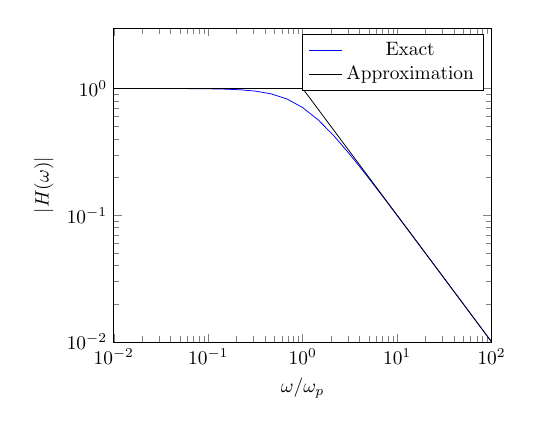
\begin{tikzpicture}[scale=0.7]
    \begin{loglogaxis}[
        xlabel=$\omega / \omega_p$, ylabel=$\abs{H(\omega)}$,
        xmin=10^(-2), xmax=10^2,
        ymin=10^(-2), ymax=3,
        % legend style={at={(1.02,1)},anchor=north west},
     ]
    \addplot [domain=10^(-2):10^2, color=blue] {1/sqrt(1 + x^2)};
    \addlegendentry{Exact};
    \addplot [domain=10^(-2):1] {1};
    \addplot [domain=1:10^(2)] {1 / x)};
    \addlegendentry{Approximation};
    \end{loglogaxis}
    \end{tikzpicture}
    \end{center}
    \end{subfigure}%
    ~ 
    \begin{subfigure}[t]{0.5\textwidth}
    \begin{center}
    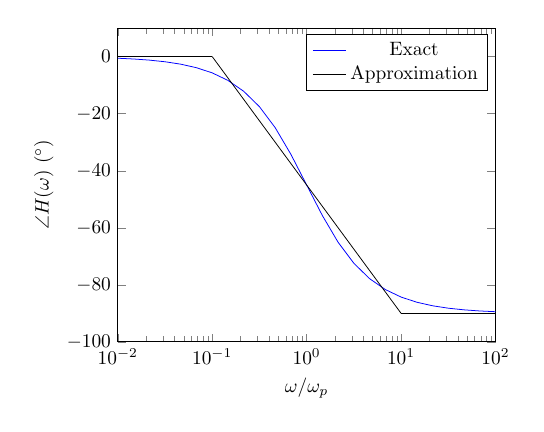
\begin{tikzpicture}[scale=0.7]
    \begin{semilogxaxis}[
        xlabel=$\omega / \omega_p$, ylabel=$\angle{H(\omega)}$ (\SI{}{\degree}),
        xmin=10^(-2), xmax=10^2,
        ymin=-100, ymax=10,
        % legend style={at={(1.02,1)},anchor=north west},
     ]
    \addplot [domain=0.01:100, color=blue] {(-1) * atan(x)};
    \addlegendentry{Exact};
    \addplot [domain=0.01:0.1] {0};
    \addplot [domain=10:100] {-90};
    \addplot [domain=0.1:10] {-45 * log10(x / 0.1)};
    \addlegendentry{Approximation};
    \end{semilogxaxis}
    \end{tikzpicture}
    \end{center}
    \end{subfigure}
\end{figure*}

Often, rather than $10^x$, you will see $10x\SI{}{\decibel}$ written instead. While we will not follow this convention, it is still important to be aware of. In particular, notice that the maximum error of our approximation to $\abs{H(\omega)}$ is $\sqrt{2} \approx \SI{3}{\decibel}$, a value that is often referred to.

We can compute the transfer function of the following high-pass filter in a similar manner, which we will do without comment:
\begin{center}
\begin{circuitikz}[american]
\draw (0, 0) to[C, C=$C$] (2, 0) to[R, l=$R$] (2, -2) node[ground] {};
\draw (2, 0) to (3, 0) node[ocirc] {} node[right] {$V_{out}$};
\draw (0, 0) node[ocirc] {} node[left] {$V_{in}$};
\end{circuitikz}
\end{center}
\[
    \implies H(\omega) = \frac{j\omega / \omega_p}{1 + j\omega / \omega_p}.
\]
Now, observe that both the numerator and the denominator vary with $\omega$. We can keep the numerator in its current form, and again approximate the denominator as either $1$ or $j \omega / \omega_p$, depending on the value of $\omega$ versus $\omega_p$. Thus, we find that
\[
    H(\omega) \approx
    \begin{cases}
        j \omega / \omega_p,                              & \text{if } \omega \ll \omega_p \\
        \frac{j\omega / \omega_p}{j\omega_p / \omega_p} = 1,   & \text{if } \omega \gg \omega_p
    \end{cases}
\]

This can be plotted as follows:
\begin{figure*}[h]
    \centering
    \begin{subfigure}[t]{0.5\textwidth}
    \begin{center}
    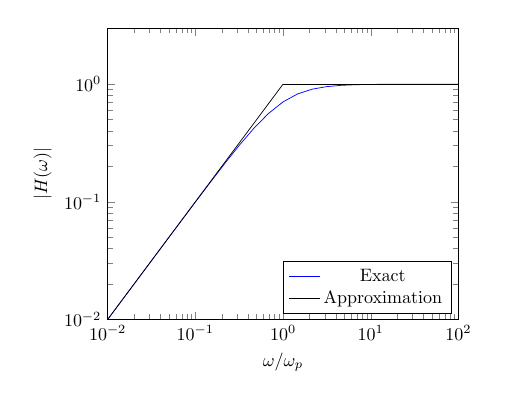
\begin{tikzpicture}[scale=0.65]
    \begin{loglogaxis}[
        xlabel=$\omega / \omega_p$, ylabel=$\abs{H(\omega)}$,
        xmin=10^(-2), xmax=10^2,
        ymin=10^(-2), ymax=3,
        legend style={at={(0.98,0.02)},anchor=south east},
     ]
    \addplot [domain=10^(-2):10^2, color=blue] {x/sqrt(1 + x^2)};
    \addlegendentry{Exact};
    \addplot [domain=10^(-2):1] {x};
    \addplot [domain=1:10^(2)] {1)};
    \addlegendentry{Approximation};
    \end{loglogaxis}
    \end{tikzpicture}
    \end{center}
    \end{subfigure}%
    ~ 
    \begin{subfigure}[t]{0.5\textwidth}
    \begin{center}
    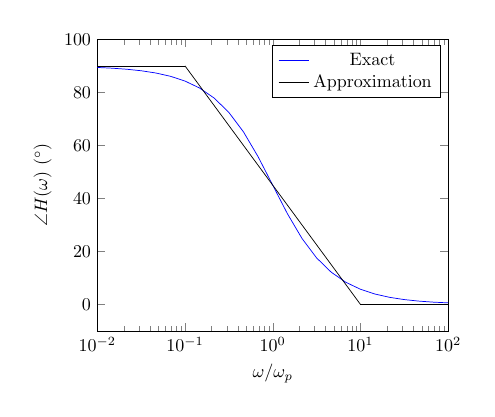
\begin{tikzpicture}[scale=0.65]
    \begin{semilogxaxis}[
        xlabel=$\omega / \omega_p$, ylabel=$\angle{H(\omega)}$ (\SI{}{\degree}),
        xmin=10^(-2), xmax=10^2,
        ymin=-10, ymax=100,
        % legend style={at={(1.02,1)},anchor=north west},
     ]
    \addplot [domain=0.01:100, color=blue] {90 - atan(x)};
    \addlegendentry{Exact};
    \addplot [domain=0.01:0.1] {90};
    \addplot [domain=10:100] {0};
    \addplot [domain=0.1:10] {90-45 * log10(x / 0.1)};
    \addlegendentry{Approximation};
    \end{semilogxaxis}
    \end{tikzpicture}
    \end{center}
    \end{subfigure}
\end{figure*}

\section{Bode Plots}
We will now consider a slightly more complex system and, in doing so, determine how to construct similar plots for more complex transfer functions. Imagine that the above two filters were placed in series, as follows:
\begin{center}
\begin{circuitikz}[american]
\draw (5, -0.5) node[op amp, yscale=-1](opamp){};
\draw (0, 0) to[R, l=$R_1$] (2, 0) to[C, l=$C_1$] (2, -2) node[ground] {};
\draw (2, 0) to (3, 0) node[ocirc] {} node[above] {$V_{center}$} to (opamp.+);
\draw (0, 0) node[ocirc] {} node[left] {$V_{in}$};
\draw (6.5, 0) to[C, C=$C_2$] (8.5, 0) to[R, l=$R_2$] (8.5, -2) node[ground] {};
\draw (8.5, 0) to (9.5, 0) node[ocirc] {} node[right] {$V_{out}$};
\draw (0, 0) node[ocirc] {} node[left] {$V_{in}$};
\draw (opamp.-) to (3.5, -1) to (3.5, -2) to (6.5, -2) to (6.5, -0.5) to (opamp.out);
\draw (6.5, -0.5) to (6.5, 0);
\end{circuitikz}
\end{center}
Notice the op-amp serving as a unity gain buffer between the two filters. It is introduced to prevent the second circuit from loading the first, since we rely on no current being drawn from the intermediate node of the first filter, as we used the voltage divider equation in calculating its behavior. Alternatively, we could choose component values of the second filter that made its impedance at all frequencies much larger than that of $C_1$, to prevent significant current from being drawn.

Let the input voltage phasor be $\tilde{V}_{in}$ at some frequency $\omega$, and let the two filters have pole frequencies $w_{p_1}$ and $w_{p_2}$ respectively. Thus, the voltage phasor at $V_{center}$ is
\[
    \tilde{V}_{center} = H_1(\omega) \tilde{V}_{in}.
\]
Since $V_{center}$ is provided as an input to the second filter, we see that the output voltage phasor $\tilde{V}_{out}$ is
\[
    \tilde{V}_{out} = H_2(\omega) \tilde{V}_{center} = H_2(\omega) H_1(\omega) \tilde{V}_{in}.
\]
Thus, the net transfer function $H(\omega)$ is
\[
    H(\omega) = H_1(\omega)H_2(\omega).
\]
More generally, placing filters in series, such that their effects are independent (either by using a buffer, or by choosing appropriate impedances) produces a circuit whose transfer function is the product of all the transfer functions of the constituent filters.

Recall that the product of two complex numbers has the properties that
\eqn{
    && \abs{z_1z_2} = \abs{z_1}\abs{z_2} \\
    && \angle{z_1z_2} = \angle{z_1} + \angle{z_2}.
}
Thus, we see that
\[
    \log{\abs{z_1z_2}} = \log{\abs{z_1}} + log{\abs{z_2}}.
\]
As a consequence, when plotting $\abs{H(\omega)}$ on a log-log plot, we can simply plot $\abs{H_1(\omega)}$ and $\abs{H_2(\omega)}$ and add them up. Similarly, when we plot $\angle{H(\omega)}$, we can again just add up $\angle{H_1(\omega)}$ and $\angle{H_2(\omega)}$. We must be careful, however, to note that in most of our plots, the $x$-axis does \emph{not} correspond to $0$, so we can't simply ``stack'' the two plots.

Let's look at a numerical example, by setting the pole frequencies of the above filter as follows:
\eqn{
    && \omega_{p_1} &= \SI{10}{\kilo\hertz} \\
    && \omega_{p_2} &= \SI{5}{\kilo\hertz}.
}
Following this procedure for amplitude (with the individual filters on the left and the result on the right), we obtain
\begin{figure}[H]
    \centering
    \begin{subfigure}{0.5\textwidth}
    \begin{center}
    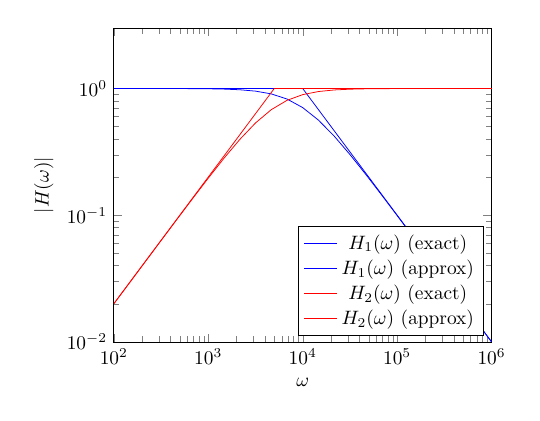
\begin{tikzpicture}[scale=0.7]
    \begin{loglogaxis}[
        xlabel=$\omega$, ylabel=$\abs{H(\omega)}$,
        xmin=10^2, xmax=10^6,
        ymin=10^(-2), ymax=3,
        legend style={at={(0.98,0.02)},anchor=south east},
     ]
    \addplot [domain=10^2:10^6, color=blue] {1/sqrt(1 + (x/10^4)^2)};
    \addlegendentry{$H_1(\omega)$ (exact)};
    \addplot [domain=10^2:10^4, color=blue, forget plot] {1};
    \addplot [domain=10^4:10^6, color=blue] {1 / (x/10^4)};
    \addlegendentry{$H_1(\omega)$ (approx)};
    
    \addplot [domain=10^2:10^6, color=red] {(x/(5 * 10^3))/sqrt(1 + (x/(5 * 10^3))^2)};
    \addlegendentry{$H_2(\omega)$ (exact)};
    \addplot [domain=10^2:5*10^3, color=red, forget plot] {(x/(5 * 10^3))};
    \addplot [domain=5*10^3:10^6, color=red] {1};
    \addlegendentry{$H_2(\omega)$ (approx)};
    
    \end{loglogaxis}
    \end{tikzpicture}
    \end{center}
    \end{subfigure}%
    ~ 
    \begin{subfigure}{0.5\textwidth}
    \begin{center}
    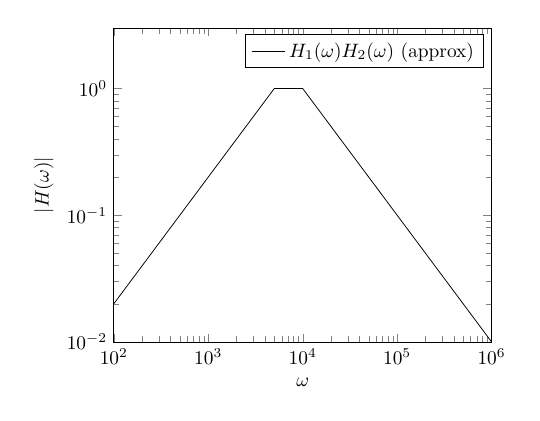
\begin{tikzpicture}[scale=0.7]
    \begin{loglogaxis}[
        xlabel=$\omega$, ylabel=$\abs{H(\omega)}$,
        xmin=10^2, xmax=10^6,
        ymin=10^(-2), ymax=3,
        % legend style={at={(1.02,1)},anchor=north west},
     ]
    
    \addplot [domain=10^2:5*10^3, forget plot] {(x/(5 * 10^3))};
    \addplot [domain=5*10^3:10^4] {1};
    \addplot [domain=10^4:10^6] {1 / (x/10^4)};
    \addlegendentry{$H_1(\omega)H_2(\omega)$ (approx)};
    
    \end{loglogaxis}
    \end{tikzpicture}
    \end{center}
    \end{subfigure}
\end{figure}

% And for phase, we similarly obtain:
% \begin{figure*}
%     \centering
%     \begin{subfigure}{0.5\textwidth}
%     \begin{center}
%     \begin{tikzpicture}[scale=0.7]
%     \begin{semilogxaxis}[
%         xlabel=$\omega$, ylabel=$\angle{H(\omega)}$ (\SI{}{\degree}),
%         xmin=10^2, xmax=10^6,
%         ymin=-100, ymax=100,
%         legend style={at={(0.98,0.02)},anchor=south east},
%      ]
%     \addplot [domain=10^2:10^6, color=blue] {90 - atan(x / 10^4)};
%     \addlegendentry{$H_1(\omega)$ (exact)};
%     \addplot [domain=10^3:10^5, forget plot] {90-45 * log10(x / 10^3)};
%     \addplot [domain=10^2:10^3, forget plot] {90};
%     \addplot [domain=10^5:10^6] {0};
%     \addlegendentry{$H_1(\omega)$ (approx)};
    
%     \addplot [domain=10^2:10^6, color=blue] {-90 + atan(x / (5 * 10^3))};
%     \addlegendentry{$H_1(\omega)$ (exact)};
%     \addplot [domain=(5 * 10^2):(5 * 10^4), forget plot] {-90 + 45 * log10(x / (5 * 10^2))};
%     \addplot [domain=10^2:(5 * 10^2), forget plot] {-90};
%     \addplot [domain=(5 * 10^4):10^6] {0};
%     \addlegendentry{$H_1(\omega)$ (approx)};
    
%     \end{semilogxaxis}
%     \end{tikzpicture}
%     \end{center}
%     \end{subfigure}%
%     ~ 
%     \begin{subfigure}{0.5\textwidth}
%     \begin{center}
%     \begin{tikzpicture}[scale=0.7]
%     \begin{semilogxaxis}[
%         xlabel=$\omega$, ylabel=$\angle{H(\omega)}$ (\SI{}{\degree}),
%         xmin=10^2, xmax=10^6,
%         ymin=-100, ymax=100,
%         legend style={at={(0.98,0.02)},anchor=south east},
%      ]
    
%     \addplot [domain=10^2:10^6, color=blue] {atan(x / (5 * 10^3)) - atan(x / 10^4)};
%     \addlegendentry{$H_2(\omega)$ (exact)};
    
%     \end{semilogxaxis}
%     \end{tikzpicture}
%     \end{center}
%     \end{subfigure}
% \end{figure*}

% A similar procedure can be conducted for phase, though it gets a little tricky when the poles are very close together, like they are in this instance.

However, we can also construct a Bode magnitude plot of a filter directly, without having to break it down into smaller filters. For the filter above, we see that
\[
    H(\omega) = H_1(\omega)H_2(\omega) = \frac{j\omega / \omega_{p_2}}{(1 + j \omega / \omega_{p_1})(1 + j \omega / \omega_{p_2})}.
\]
Now, imagine that we didn't notice that this filter could be written as the product of a low-pass and high-pass filter. So long as the numerator and denominator are both factorized with factors in the form $(1 + j\omega / \omega_k)$ or $j\omega / \omega_k$, we can plot the function. Without loss of generality, assume that $\omega_{p_1} > \omega_{p_2}$. There are three regions to consider: $\omega < \omega_{p_2}$, $\omega_{p_2} < \omega < \omega_{p_1}$, and $\omega_{p_1} < \omega$. For each of these regions, we may make the approximations:
\[
    H(\omega) =
    \begin{cases}
        \frac{j\omega / \omega_{p_2}}{(1 + j \omega / \omega_{p_1})(1 + j \omega / \omega_{p_2})} \approx \frac{j\omega / \omega_{p_2}}{(1)(1)} = j\omega / \omega_{p_2},                              & \text{if } \omega < \omega_{p_2} \\
         \frac{j\omega / \omega_{p_2}}{(1 + j \omega / \omega_{p_1})(1 + j \omega / \omega_{p_2})} \approx \frac{j\omega / \omega_{p_2}}{(1)(j\omega / \omega_{p_2})} = 1,   & \text{if } \omega_{p_2} < \omega < \omega_{p_1} \\
        \frac{j\omega / \omega_{p_2}}{(1 + j \omega / \omega_{p_1})(1 + j \omega / \omega_{p_2})} \approx \frac{j\omega / \omega_{p_2}}{(j\omega / \omega_{p_1})(j\omega / \omega_{p_2})} = \frac{1}{j\omega / \omega_{p_2}},   & \text{if } \omega > \omega_{p_1}
    \end{cases}
\]
Notice that we are essentially ``sweeping'' $\omega$ from $0$ to $\infty$ through each of the pole frequencies (actually, if an $\omega_k$ is in the numerator, we call it a \emph{zero}, not a pole) and seeing which parts of each of the terms in our factorization dominate. We can then plot this function directly, to obtain the same results as from earlier.

\section{LC Filters}
Now, we will return to the final class of L-filters that we skipped in the previous lecture: \emph{LC Filters}, composed of a capacitor and an inductor. Consider the following circuit:
\begin{center}
\begin{circuitikz}[american]
\draw (0, 0) to[C, C=$C$] (2, 0) to[L, l=$L$] (2, -2) node[ground] {};
\draw (2, 0) to (3, 0) node[ocirc] {} node[right] {$V_{out}$};
\draw (0, 0) node[ocirc] {} node[left] {$V_{in}$};
\end{circuitikz}
\end{center}
Using the voltage divider equation, we can quickly see that
\[
    H(\omega) = \frac{j\omega L}{j\omega L + \frac{1}{j\omega C}} = \frac{-\omega^2 LC}{1 - \omega^2 LC}.
\]
Notice that this transfer function lacks any imaginary component, so an LC filter will never introduce a phase shift (except possibly for a \SI{180}{degree} one, since that just flips the amplitude of a signal). However, also notice that as the denominator lacks an imaginary portion, it will go to zero at $\omega_n = \frac{1}{\sqrt{LC}}$, known as the \emph{resonant frequency} of the circuit. At that point, $H(\omega) \to \pm\infty$, which is unphysical. We will therefore have to analyze its behavior more closely at that point.

First, though, let's look at the extreme values of $\omega$, like we have before, to obtain a linear approximation of the transfer function of this circuit. Rewriting $H(\omega)$ in terms of $\omega_n$, we obtain
\[
    H(\omega) = \frac{-\omega^2 / \omega_n^2}{1 - \omega^2 / \omega_n^2}.
\]
We see that
\[
    H(\omega) =
    \begin{cases}
        \frac{-\omega^2LC}{1 - \omega^2 / \omega_n^2} \approx -\omega^2 / \omega_n^2, & \text{if } \omega \ll \omega_n \\
        \frac{-\omega^2LC}{1 - \omega^2 / \omega_n^2} \approx 1,   & \text{if } \omega \gg \omega_n
    \end{cases}
\]
Plotting this approximation to $\abs{H(\omega)}$ on a log-log scale alongside the exact plot, we obtain
\begin{center}
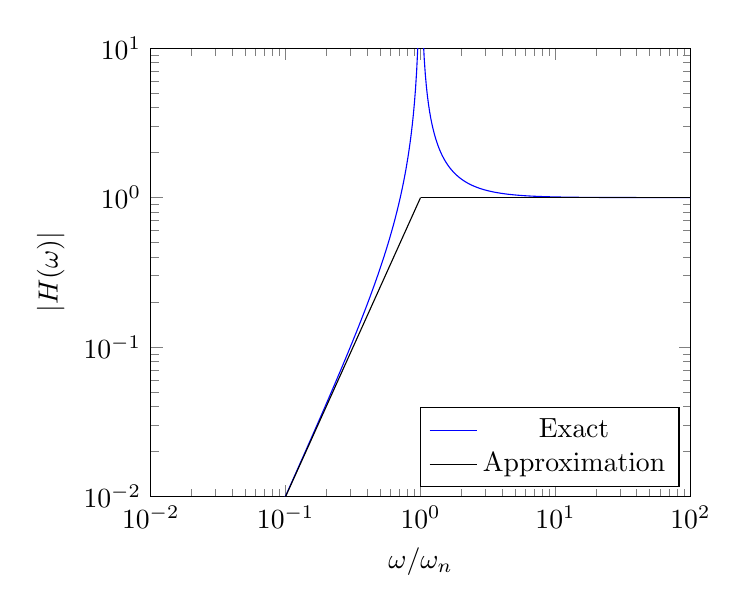
\begin{tikzpicture}
\begin{loglogaxis}[
    xlabel=$\omega / \omega_n$, ylabel=$\abs{H(\omega)}$,
    xmin=10^(-2), xmax=10^2,
    ymin=10^(-2), ymax=10^1,
    legend style={at={(0.98,0.02)},anchor=south east},
 ]
\addplot [domain=10^(-2):10^2, color=blue, samples=500] {x^2 / abs(1 - x^2)};
\addlegendentry{Exact};
\addplot [domain=10^(-2):1] {x^2};
\addplot [domain=1:10^(2)] {1};
\addlegendentry{Approximation};
\end{loglogaxis}
\end{tikzpicture}
\end{center}
Notice the spike to infinity at $\omega_n$. Similarly, plotting our approximations to $\angle{H(\omega)}$ alongside the exact plot, we obtain:
\begin{center}
\begin{tikzpicture}
\begin{semilogxaxis}[
    xlabel=$\omega / \omega_n$, ylabel=$\angle{H(\omega)}$ (\SI{}{\degree}),
    xmin=10^(-2), xmax=10^2,
    ymin=-100, ymax=100,
    legend style={at={(1.02,1)},anchor=north west},
 ]
\addplot [domain=0.01:1, color=blue, forget plot] {-90};
\addplot [domain=1:100, color=blue] {90};
\addplot [color=blue, dashed, forget plot] coordinates {(1, -90) (1, 90)};
\addlegendentry{Exact};
\addplot [domain=0.01:0.1] {-90};
\addplot [domain=10:100] {90};
\addplot [domain=0.1:10] {90 * log10(x / 0.1) - 90};
\addlegendentry{Approximation};
\end{semilogxaxis}
\end{tikzpicture}
\end{center}
Notice that there is a discontinuity about $\omega_n$, with $\abs{H(\omega)}$ going to infinity, and $\angle{H(\omega)}$ rapidly jumping from $-1$ to $1$. Clearly, something is wrong with our model of this filter. We will address this by first considering the phenomenon of \emph{resonance}.

\section{Resonance}
Consider the following LC circuit, known as an \emph{LC tank circuit}:
\begin{center}
\begin{circuitikz}[american]
\draw (0, 0) to (2, 0) to[L, l=$L$, i=$I$] (2, -2) node[ground] {};
\draw (1, 0) to[C, a=$C$] (1, -2) to (2, -2);
\draw (0, 0) node[ocirc] {} node[left] {$V_{in}$};
\end{circuitikz}
\end{center}

Initially, we will leave $V_{in}$ floating, to study the natural behavior of this circuit. Notice that we cannot use phasor analysis to solve for this behavior, since we do not know the circuit's frequency of oscillation. Instead, we will write down the differential equations directly, as follows:
\eqn{
    && L\frac{\dI}{\dt} &= V_{in} \\
    && -C\frac{\diff V_{in}}{\dt} &= I.
}
Eliminating $I$, we find that
\eqn{
    && -C \frac{\diff^2 V_{in}}{\dt^2} &= \frac{\dI}{\dt} \\
    \thus -LC\frac{\diff^2 V_{in}}{\dt^2} &= V_{in}.
}
We do not yet have the techniques to solve this equation directly, though we will develop them in future lectures. Instead, at this moment we will simply conjecture a solution of the following form:
\[
    V_{in} = V_0 \sin(\omega t + \phi),
\]
where $V_0$, $\omega$, and $\phi$ are all parameters to be determined. Substituting into our differential equation, we find that
\eqn{
    && \frac{\diff V_{in}}{\dt} &= \omega V_0 \cos(\omega t + \phi) \\
    \thus \frac{\diff^2 V_{in}}{\dt} &= -\omega^2 V_0 \sin(\omega t + \phi) \\
    \thus \omega^2LCV_0 \sin(\omega t + \phi) &= V_0 \sin(\omega t + \phi) \\
    \thus \omega &= \frac{1}{\sqrt{LC}}.
}
Notice that no constraints were imposed on $V_0$, indicating that this circuit may freely resonate with unbounded amplitude, despite not being driven by a voltage source. Also notice that the natural resonant frequency $\omega$ is the same as the frequency $\omega_n$ from our earlier discussion.

Now, imagine that we drive $V_{in}$ with a voltage phasor $\tilde{V}$ at frequency $\omega _n$. Performing frequency analysis, we find that the equivalent impedance from $V_{in}$ to ground is
\[
    Z_{eq} = (j\omega L) || \left(\frac{1}{j\omega C}\right) = \frac{1}{\frac{1}{j\omega L} + j\omega C} = \frac{j\omega L}{1 - \omega^2 LC}.
\]
Linearly approximating $Z_{eq}$ for extreme values of $\omega$, we find that
\[
    H(\omega) =
    \begin{cases}
        j\omega L, & \text{if } \omega \ll \omega_n \\
        \frac{1}{j\omega C}, & \text{if } \omega \gg \omega_n
    \end{cases}.
\]
Plotting these linear approximations alongside the exact function for $\abs{Z_{eq}}$, we obtain
\begin{center}
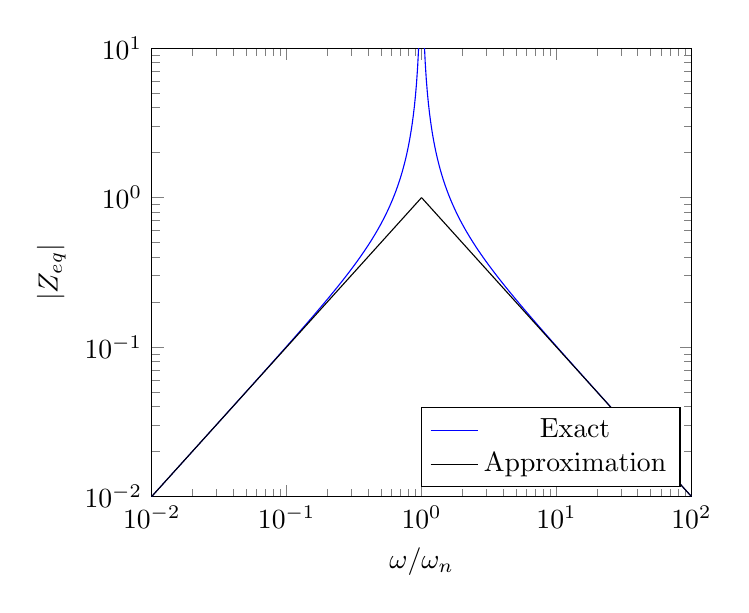
\begin{tikzpicture}
\begin{loglogaxis}[
    xlabel=$\omega / \omega_n$, ylabel=$\abs{Z_{eq}}$,
    xmin=10^(-2), xmax=10^2,
    ymin=10^(-2), ymax=10^1,
    legend style={at={(0.98,0.02)},anchor=south east},
 ]
\addplot [domain=10^(-2):10^2, color=blue, samples=500] {x / abs(1 - x^2)};
\addlegendentry{Exact};
\addplot [domain=10^(-2):1] {x};
\addplot [domain=1:10^(2)] {1 / x};
\addlegendentry{Approximation};
\end{loglogaxis}
\end{tikzpicture}
\end{center}
Notice that our approximation again breaks down near the resonant frequency $\omega_n$, where at that point $Z_{eq} \to \infty$.

As an infinite impedance represents an open circuit, we see that no current will be drawn from $V_{in}$ or sent to ground. Nevertheless, since $V_{in}$ is oscillating, there must be current flowing within the LC tank, with the capacitor charging and discharging - in essence, this current indicates some stored energy oscillating between the capacitor and inductor\footnote{Hence the term LC ``tank''.}.

In a similar manner, a current source at the resonant frequency $omega = 1 / \sqrt{LC}$ driving an inductor and capacitor in series will not produce any voltage, as shown:
\begin{center}
\begin{circuitikz}[american]
\draw (0, 0) to[current source, l=$I_0\cos{\omega t}$, v=$\SI{0}{\volt}$] (0, 2) to[L, l=$L$] (2, 2) to[C, l=$C$] (2, 0) to (0, 0) node[ground]{};
\end{circuitikz}
\end{center}
We can see this by computing the equivalent impedance of the inductor and capacitor in series, to obtain
\[
    Z_{eq} = j\omega L + \frac{1}{j\omega C} = \frac{j\omega L}{\sqrt{LC}} + \frac{\sqrt{LC}}{j \omega C} = j\omega\left(\sqrt{\frac{L}{C}} - \sqrt{\frac{L}{C}}\right) = 0.
\]
Thus, it is as if we shorted the two terminals of the current source together, so of course no voltage can ever exist across them.

\section{RLC Circuits}
Of course, recall that an inductor is really a long coil of wire, which has some internal resistance. Thus, a more accurate model of a real inductor should include a resistor in series, as shown:
\begin{center}
\begin{circuitikz}[american]
\draw (0, 0) node[ocirc]{} to[L] (2, 0) to[R] (4, 0) node[ocirc]{};
\end{circuitikz}
\end{center}

Recall from before that an inductor and capacitor, placed in series, exhibit zero overall impedance when driven at their resonant frequency. But now, we really obtain the circuit
\begin{center}
\begin{circuitikz}[american]
    \draw (0, 0) node[ocirc]{} to[L, l=$L$] (2, 0) to[R, l=$R$] (4, 0) to[C, l=$C$] (6, 0) node[ocirc]{};
\end{circuitikz}
\end{center}
with equivalent resistance (at $\omega = 1/\sqrt{LC}$)
\[
    Z_{eq} = j\omega L + R + \frac{1}{j\omega C} = R + \frac{j L}{\sqrt{LC}} + \frac{\sqrt{LC}}{j C} = R +  j\left(\sqrt{\frac{L}{C}} - \sqrt{\frac{L}{C}}\right) = R.
\]
Thus, even at the resonant frequency, there will be some resistance $R$ - we will never hit $0$ (or, as it turns out, infinite) impedance. 

We will now calculate a linear approximation for our new $Z_{eq}$ (by considering extreme values of $\omega$, as we have done before) to obtain:
\[
    Z_{eq}(\omega) \approx
    \begin{cases}
        \frac{1}{j\omega C}, & \text{if } \omega \ll \omega_n \\
        j\omega L,   & \text{if } \omega \gg \omega_n
    \end{cases}
\]

Plotting both our approximation and the exact values of $\abs{Z_{eq}}$ for various values of $\omega$, along with a plot of the impedance of a real inductor (i.e. an inductor and resistor in series) we obtain the plot (for $R = \SI{100}{\milli\ohm}$, $L = \SI{1}{\henry}$, $C=\SI{1}{\farad}$):
\begin{center}
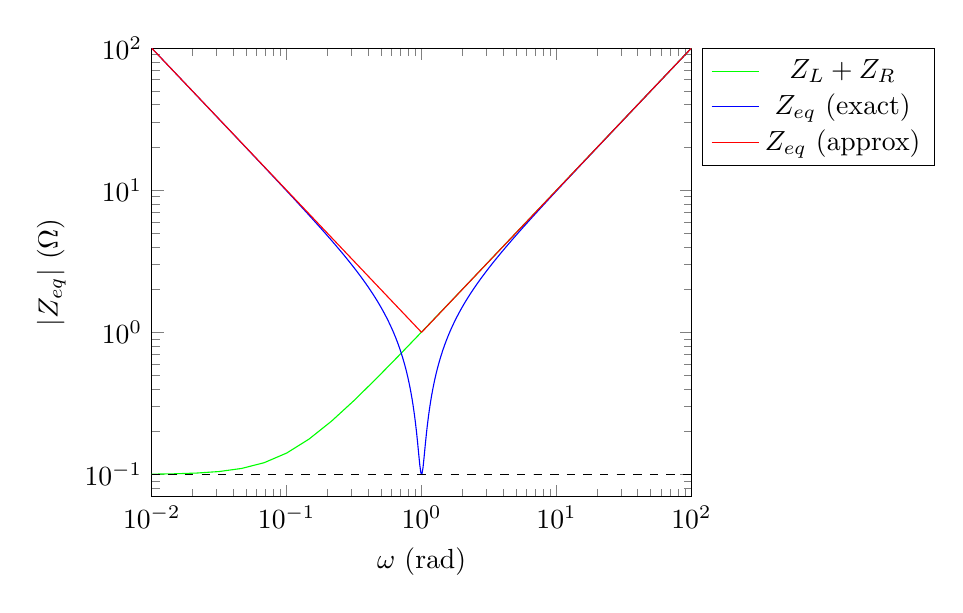
\begin{tikzpicture}
\begin{loglogaxis}[
    xlabel=$\omega$ (\SI{}{\radian}), ylabel=$\abs{Z_{eq}}$ (\SI{}{\ohm}),
    xmin=10^(-2), xmax=10^2,
    ymin=0.7*10^(-1), ymax=10^2,
    legend style={at={(1.02,1)},anchor=north west},
 ]
\addplot [domain=10^(-2):10^2, color=green] {sqrt(0.1^2 + x^2)};
\addlegendentry{$Z_{L} + Z_{R}$};
\addplot [domain=10^(-2):10^2, color=blue, samples=500] {sqrt(0.1^2 + (x - (1/x))^2)};
\addlegendentry{$Z_{eq}$ (exact)};
\addplot [domain=10^(-2):1, color=red, forget plot] {1 / x};
\addplot [domain=1:10^2, color=red] {x};
\addlegendentry{$Z_{eq}$ (approx)};
\addplot [domain=10^(-2):10^2, dashed, forget plot] {0.1};
% \addplot [domain=10^(-2):1] {x};
% \addplot [domain=1:10^(2)] {1 / x};
% \addlegendentry{Approximation};
\end{loglogaxis}
\end{tikzpicture}
\end{center}
Notice that our model of the inductor now flattens out to approach an asymptote of $R$ as $\omega \to 0$, so it no longer lets low-frequency signals through perfectly. As a consequence, $Z_{eq}$ never reaches $0$, since the resistance of the inductor will contribute to $Z_{eq}$ at all frequencies.

Observe the sharp drop in impedance near the resonant frequency, with the impedance plunging from what we expect from our linear models all the way down to $R$. We quantify the ``sharpness'', or \emph{quality}, of this drop using the \emph{Q-factor}, which is the ratio between the expected impedance at resonance using a linear model, and the actual resonance. Here, we can compute the Q-factor to be
\[
    Q = \frac{\sqrt{\frac{L}{C}}}{R} = \frac{1}{R C / \sqrt{LC}} = \frac{1}{\omega_nRC},
\]
since from our linear model $Z_{eq}(\omega_n) = \sqrt{L / C}$, when in reality $Z_{eq}(\omega_n) = R$.

Another way of quantifying the sharpness of this drop is known as the \emph{bandwidth} $B$, and is defined to be the maximum value such that
\[
    \abs{Z_{eq}}(\omega_n \pm B / 2) \le \sqrt{2} (\abs{Z_{eq}}(\omega_n)).
\]
In other words, it describes how far the frequency $\omega$ can deviate from $\omega_n$ before the impedance rises significantly. 

Now, we can solve for $B$. Let $\omega_1 = \omega_n - B/2$. Thus,
\eqn{
    && \abs{Z_{eq}}\left(\omega - \frac{B}{2}\right) &= \sqrt{2} (\abs{Z_{eq}}(\omega_n)) \\
    \thus \sqrt{R^2 + (\omega_1 L - \frac{1}{\omega_1 C})^2} &= R\sqrt{2} \\
    \thus R^2 + (\omega_1 L - \frac{1}{\omega_1 C})^2 &= 2R^2 \\
    \thus \omega L - \frac{1}{\omega_1 C} &= -R \\
    \thus \omega_1^2 L + \omega_1 R - \frac{1}{C} &= 0 \\
    \thus \omega_1 &= \frac{-R + \sqrt{R^2 + 4L / C}}{2L} \\
    &&&= -\frac{R}{2L} + \sqrt{\frac{R^2}{4L^2} + \frac{1}{LC}} \\
    &&&= \frac{1}{\sqrt{LC}} \left(-\frac{R\sqrt{C}}{2\sqrt{L}} + \sqrt{1 + \frac{R^2C}{L}} \right) \\
}
Let $\omega_2 = \omega_n + B/2$. A very similar calculation will demonstrate that
\[
    \omega_2 = \frac{1}{\sqrt{LC}} \left(\frac{R\sqrt{C}}{2\sqrt{L}} + \sqrt{1 + \frac{R^2C}{L}} \right).
\]
Thus, we see that
\eqn{
    && B &= \omega_2 - \omega_1 \\
    &&&= \frac{1}{\sqrt{LC}} \left(\frac{R\sqrt{C}}{\sqrt{L}} \right) \\
    &&&= w_n^2 RC \\
    &&&= \frac{w_n}{Q}.
}
Intuitively, this result is stating that the bandwidth and the Q-factor have an inverse relationship, which is to be expected.

Typically, LC Q-factors are of the order of $100$, which is much better than the filter we created by chaining low-pass and high-pass filters. Thus, LC filters are typically used when a \emph{band-pass filter} is required, to select a signal of a particular frequency despite the presence of noise at other frequencies.

\section{RLC Filters}
We will now return to our LC tank circuit. Including the resistance of the inductor, we obtain:
\begin{center}
\begin{circuitikz}[american]
\draw (0, 0) to (2, 0) to[R, l=$R$] (2, -2) to[L, l=$L$] (2, -4) node[ground] {};
\draw (1, 0) to[C, a=$C$] (1, -4) to (2, -4);
\draw (0, 0) node[ocirc] {} node[left] {$V_{in}$};
\end{circuitikz}
\end{center}
Recall that, without the inductor's internal resistance, this circuit provided an infinite impedance between $V_{in}$ and ground at resonance. Now, however, we can compute its impedance at some frequency $\omega$ to be
\eqn{
    && Z_{eq} &= Z_C || (R + Z_L) \\
    &&&= \frac{1}{j\omega C + \frac{1}{R + j\omega L}} \\
    &&&= \frac{R + j\omega L}{1 + j\omega RC - \omega^2 LC} \\
    &&&= (R + j\omega L) \left(\frac{1}{j\omega C} \right) \frac{1}{R + j\omega L + \frac{1}{j\omega C}} \\
    &&&= (Z_R + Z_L) Z_C \frac{1}{R + j\omega L + \frac{1}{j\omega C}}.
}
Notice that the first term is the impedance of a real inductor, the second term is the impedance of an inductor, and the final term is the reciprocal of the impedance of an RLC series circuit. Discarding the last term, we can construct a linear approximation in the standard fashion, with $Z_{eq}$ modelled by the capacitor at low frequencies and by the inductor at high frequencies. Plotting both the exact and approximate $\abs{Z_{eq}}$ against $\omega$ for $R = \SI{100}{\milli\ohm}$, $L = \SI{1}{\henry}$, we obtain
\begin{center}
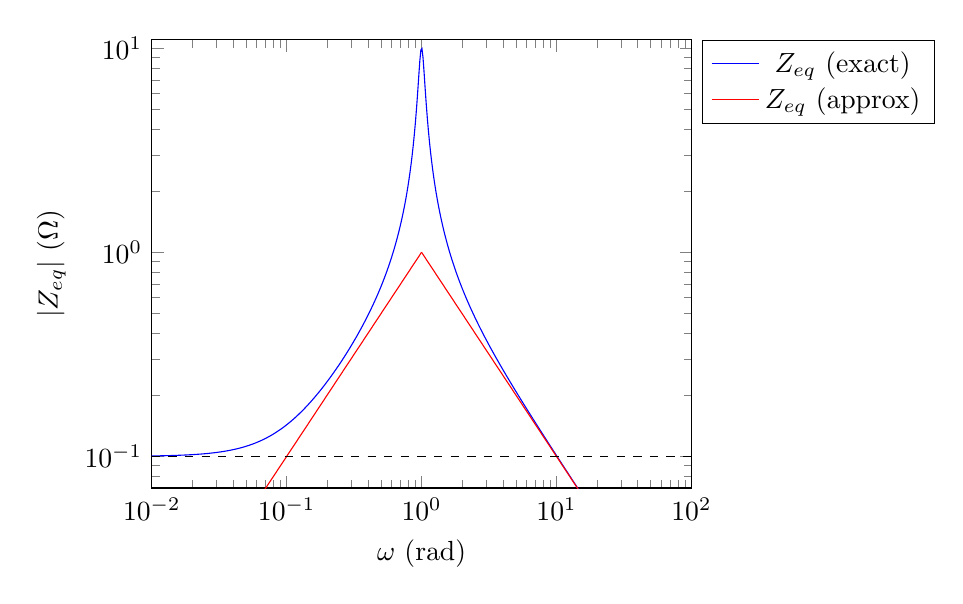
\begin{tikzpicture}
\begin{loglogaxis}[
    xlabel=$\omega$ (\SI{}{\radian}), ylabel=$\abs{Z_{eq}}$ (\SI{}{\ohm}),
    xmin=10^(-2), xmax=10^2,
    ymin=0.7*10^(-1), ymax=1.1*10,
    legend style={at={(1.02,1)},anchor=north west},
 ]
\addplot [domain=10^(-2):10^2, color=blue, samples=500] {(sqrt(0.1^2 + x^2) / x) / sqrt(0.1^2 + (x - 1/x)^2)};
\addlegendentry{$Z_{eq}$ (exact)};
\addplot [domain=1:10^2, color=red, forget plot] {1 / x};
\addplot [domain=10^(-2):1, color=red] {x};
\addlegendentry{$Z_{eq}$ (approx)};
\addplot [domain=10^(-2):10^2, dashed, forget plot] {0.1};
% \addplot [domain=10^(-2):1] {x};
% \addplot [domain=1:10^(2)] {1 / x};
% \addlegendentry{Approximation};
\end{loglogaxis}
\end{tikzpicture}
\end{center}
It can be shown, though we will not do so, that the peak of $\abs{Z_{eq}}$ here is a further factor of $Q$ above the linear approximation (so it equals $Q^2R$), just like how in the RLC series circuit the minimum was a factor of $Q$ below the linear approximation. The key idea here is that we have produced a circuit with high impedance only very near a particular frequency $\omega_n$. Thus, we can finally construct an RLC filter as follows:
\begin{center}
\begin{circuitikz}[american]
\draw (-2, 0) node[ocirc]{} node[left]{$V_{in}$} to[R, l=$R_{big}$] (0, 0) to (2, 0) to[R, l=$R$] (2, -2) to[L, l=$L$] (2, -4) node[ground] {};
\draw (1, 0) to[C, a=$C$] (1, -4) to (2, -4);
\draw (2, 0) to (3, 0) node[ocirc] {} node[right] {$V_{out}$};
\end{circuitikz}
\end{center}
Here, $R_{big}$ is greater than the impedance of the LC tank away from $\omega_n$ (so $R_{big} \gg R$). Thus, at most frequencies $\omega$, the LC tank will serve as a low-impedance path to ground, so those frequencies will be greatly attenuated at $V_{out}$. However, near $\omega_n$, the impedance of the LC tank will rise significantly, so signals at that frequency will experience practically no attenuation at $V_{out}$ and so will pass straight through.

Thus, we have finally developed a \emph{band-pass filter} that did not require us to chain many low- and high-pass filters together, and that can be produced with a very large Q-factor.

\end{document}
